\documentclass[12pt,letterpaper]{article}

\usepackage{times}
\usepackage{graphicx}
\graphicspath{ {./images/} }
\usepackage{amsmath}
\usepackage{amssymb}
\usepackage{parskip}
\usepackage{booktabs}
\usepackage[ruled,vlined]{algorithm2e}

\title{3-Dimensional Transformations}
\author{Manny Barreto, Will DiBiagio, Alex Wong}
\date{}

\begin{document}

\maketitle

\section{Preliminaries}
\subsection{Matrx Inverse}
A matrix is said to be invertible if and only if it satisfy the following constraint:

\begin{equation}
   AB = BA = I
\end{equation}

In which case $B$ is the inverse of $A$, and we can write $B = A^{-1}$. We can equivalently say that $A$ is the inverse of $B$ and write $A = B^{-1}$. Hence, we can write:

\begin{equation}
   AA^{-1} = BB^{-1} = I
\end{equation}

Suppose the matrix $A$ performs a transformation. Since the identity matrix signifies an identity transformation (i.e. nothing has changed $AI = A$), $AA^{-1} = I$ suggests that $A^{-1}$ ``undos'' the transformation.

To compute the inverse of a matrix, we can perform Gauss-Jordan elimination (a method of solving a system of linear equations). Gauss-Jordan elimination allow us to perform a set of actions known as elementary row operations:
\begin{enumerate}
    \item Adding rows
    \item Swapping rows
    \item Multiplying rows by a scalar
\end{enumerate}

\newpage

We begin with a matrix that we would like to find the inverse of:

\begin{equation}
    A = \begin{bmatrix}
        3 & 0 &  2 \\
        2 & 0 & -2 \\
        0 & 1 & 1
        \end{bmatrix}
\end{equation}

We now concatenate it with the identity matrix $I$ to create an augmented matrix $[A | I]$ with the goal of performing a set of elementary row operations to transform the augmented matrix into the form $[I|A^{-1}]$ :

\begin{equation}
    \left[\begin{array}{ccc|ccc}
    3 & 0 &  2 & 1 & 0 & 0 \\
    2 & 0 & -2 & 0 & 1 & 0 \\
    0 & 1 &  1 & 0 & 0 & 1
    \end{array}\right]
\end{equation}

We start by eliminating the 2 from the first row by adding the second to the first:

\begin{equation}
    \left[\begin{array}{ccc|ccc}
    3+2 & 0     &  2-2  & 1     & 0+1   & 0 \\
    2   & 0     & -2    & 0     & 1     & 0 \\
    0   & 1     &  1    & 0     & 0     & 1
    \end{array}\right]
    =
    \left[\begin{array}{ccc|ccc}
    5   & 0     &  0    & 1     & 1     & 0 \\
    2   & 0     & -2    & 0     & 1     & 0 \\
    0   & 1     &  1    & 0     & 0     & 1
    \end{array}\right]
\end{equation}

We can divide the first row by 5 to get the first 1 of the identity:

\begin{equation}
    \left[\begin{array}{ccc|ccc}
    5/5 & 0     &  0    & 1/5   & 1/5   & 0 \\
    2   & 0     & -2    & 0     & 1     & 0 \\
    0   & 1     &  1    & 0     & 0     & 1
    \end{array}\right]
    =
    \left[\begin{array}{ccc|ccc}
    1   & 0     &  0    & 1/5   & 1/5   & 0 \\
    2   & 0     & -2    & 0     & 1     & 0 \\
    0   & 1     &  1    & 0     & 0     & 1
    \end{array}\right]
\end{equation}

We can now use the first row to eliminate everything in the first column:

\begin{equation}
    \left[\begin{array}{ccc|ccc}
    1   & 0     &  0    & 1/5   & 1/5   & 0 \\
    0   & 0     & -2    & -2/5  & 3/5   & 0 \\
    0   & 1     &  1    & 0     & 0     & 1
    \end{array}\right]
\end{equation}

\newpage

We can now divide the second row by 2:

\begin{equation}
    \left[\begin{array}{ccc|ccc}
    1   & 0     &  0    & 1/5   & 1/5   & 0 \\
    0   & 0     & -2/2  & -2/10 & 3/10  & 0 \\
    0   & 1     &  1    & 0     & 0     & 1
    \end{array}\right]
    =
    \left[\begin{array}{ccc|ccc}
    1   & 0     &  0    & 1/5   & 1/5   & 0 \\
    0   & 0     & -1    & -2/10 & 3/10  & 0 \\
    0   & 1     &  1    & 0     & 0     & 1
    \end{array}\right]
\end{equation}

We can multiply the second row by -1 and swap the third and second row and multiply to get the last diagonal of the identity:

\begin{equation}
    \left[\begin{array}{ccc|ccc}
    1   & 0     &  0    & 1/5   & 1/5   & 0 \\
    0   & 1     &  1    & 0     & 0     & 1 \\
    0   & 0     &  1    & 2/10  & -3/10 & 0
    \end{array}\right]
\end{equation}

And lastly use the third row to eliminate the second row:

\begin{equation}
    \left[\begin{array}{ccc|ccc}
    1   & 0     &  0    & 1/5   & 1/5   & 0 \\
    0   & 1     &  0    & -2/10 & 3/10  & 1 \\
    0   & 0     &  1    & 2/10  & -3/10 & 0
    \end{array}\right]
\end{equation}

Our inverse is now:
\begin{equation}
    A^{-1} = \begin{bmatrix}
        1/5   & 1/5   & 0 \\
        -2/10 & 3/10  & 1 \\
        2/10  & -3/10 & 0
        \end{bmatrix}
\end{equation}

We can now apply this method to generically find the inverse of our transformation matrices. For example, let's perform this to a translation matrix $T_{a,b}$ to find its inverse $T^{-1}$:

\begin{equation}
    \left[\begin{array}{ccc|ccc}
    1 & 0 &  a & 1 & 0 & 0 \\
    0 & 1 &  b & 0 & 1 & 0 \\
    0 & 0 &  1 & 0 & 0 & 1
    \end{array}\right]
\end{equation}

We can eliminate the second row by subtracting $b$ times the third row:

\begin{equation}
    \left[\begin{array}{ccc|ccc}
    1 & 0 &  a & 1 & 0 & 0 \\
    0 & 1 &  0 & 0 & 1 & -b \\
    0 & 0 &  1 & 0 & 0 & 1
    \end{array}\right]
\end{equation}

And similarly eliminate the first row by subtracting $a$ times the first:

\begin{equation}
    \left[\begin{array}{ccc|ccc}
    1 & 0 &  0 & 1 & 0 & -a \\
    0 & 1 &  0 & 0 & 1 & -b \\
    0 & 0 &  1 & 0 & 0 & 1
    \end{array}\right]
\end{equation}

The inverse of $T_{a,b}$ is:

\begin{equation}
    T^{-1} = \begin{bmatrix}
        1   & 0     & -a \\
        0   & 1     & -b \\
        0   & 0     & 1
        \end{bmatrix}
\end{equation}

\subsection{Cross Product}
The cross ($\times$) of two vectors is defined in 3-dimensional space. The cross of $\overrightarrow{a}$ and $\overrightarrow{b}$ will give us a new vector $\overrightarrow{c}$ that is orthogonal or perpendicular to both $\overrightarrow{a}$ and $\overrightarrow{b}$.

\begin{equation}
   \overrightarrow{c} = \overrightarrow{a} \times \overrightarrow{b} = ||\overrightarrow{a}||||\overrightarrow{b}||\text{sin}(\theta)\overrightarrow{n}
\end{equation}

where $\overrightarrow{n}$ is the normal vector to $\overrightarrow{a}$ and $\overrightarrow{b}$, and $\theta$ is the angle between $\overrightarrow{a}$ and $\overrightarrow{b}$.

We can redefine this using the components of $\overrightarrow{a} = <a_x, a_y, a_z>$ and \\ $\overrightarrow{b} = <b_x, b_y, b_z>$ by computing each component using the product of the cross of the other components:

\begin{equation}
   \overrightarrow{c} = \overrightarrow{a} \times \overrightarrow{b} =
   \left|\begin{array}{ccc}
    x & y &  z \\
    a_x & a_y & a_z \\
    b_x & b_y & b_z
    \end{array}\right| =
    \begin{bmatrix}
        a_y b_z - a_z b_y \\
        - a_x b_z + a_z b_x \\
        a_x b_y - a_y b_x
    \end{bmatrix}
\end{equation}

Note that $\overrightarrow{a} \times \overrightarrow{b}$ is orthogonal to both $\overrightarrow{a}$ and $\overrightarrow{b}$; however, $\overrightarrow{a}$ and $\overrightarrow{b}$ may not be orthogonal themselves. Additionally, the cross between a vector $\overrightarrow{a}$ and itself is 0, $\overrightarrow{a} \times \overrightarrow{a} = 0$.

Note that the cross product of two vectors $\overrightarrow{a} \times \overrightarrow{b}$ can be visualized by the right hand rule given by index ($\overrightarrow{a}$), middle ($\overrightarrow{b}$) and the resulting vector thumb ($\overrightarrow{a} \times \overrightarrow{b}$).

Note: the computation of the cross product is essentially the determinant. The determinant of a matrix $det(A)$ is the volume of a parallelepiped spanned by the column or row vectors of the matrix.

\begin{equation}
   det(A) = x(a_y b_z - a_z b_y) + -y(a_x b_z - a_z b_x) + z (a_x b_y - a_y b_x)
\end{equation}

\section{Defining a 3D Coordinate Frame}
Similar to a 2D coordinate frame, a 3D coordinate frame can be defined using three vectors (axes) and a point (origin). We begin by defining a 3D coordinate frame using vectors  $\overrightarrow{u}$, $\overrightarrow{v}$ $\overrightarrow{w}$ and the origin $O$. To define a point $p$ in this 3D coordinate frame, we can express $p$ using coefficients $x$, $y$ and $z$:

\begin{equation}
   p = x\overrightarrow{u} + y\overrightarrow{v} + z\overrightarrow{w} + O
\end{equation}

with $\overrightarrow{u}$, $\overrightarrow{v}$ and $\overrightarrow{w}$ as unit vectors. To keep our notation in homogeneous coordinate, we will expand our matrices to 4-dimensional (4D) denoted as $[x, y, z, 1]$

We now write $p = x\overrightarrow{u} + y\overrightarrow{v} + z\overrightarrow{w} + O$ into their vector forms using homogeneous coordinates:

\begin{equation}
    p = \begin{bmatrix}
        x & y & z & 1
    \end{bmatrix}
    \begin{bmatrix}
        \overrightarrow{u} \\
        \overrightarrow{v} \\
        \overrightarrow{w} \\
        O
    \end{bmatrix}
    = x\overrightarrow{u} + y\overrightarrow{v} + z\overrightarrow{w} + O
\end{equation}

\newpage

\section{3D Transformations}
We may place objects in this 3D space as points or sets of points. Our goal is to perform transformations in 3D space to some point $p = (x, y, z)$.

\subsection{Translation}
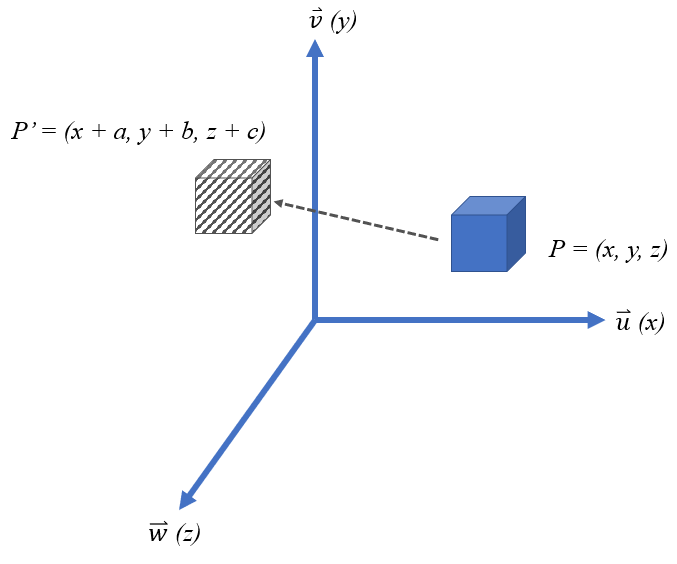
\includegraphics[scale=0.75]{translation}
We want to move the point $p = (x, y, z)$ to a new position $p' = (x+a, y+b, z+c)$. This naturally becomes a mapping from $[x, y, c, 1] \rightarrow [x+a, y+b, z+c, 1]$. We will need a $4 \times 4$ matrix:

\begin{equation}
    T_{a, b, c} = \begin{bmatrix}
        1 & 0 & 0 & a \\
        0 & 1 & 0 & b \\
        0 & 0 & 1 & c \\
        0 & 0 & 0 & 1
    \end{bmatrix}
\end{equation}

This matrix will perform a 3D translation to any point $p = (x, y, z)$ to a new location with offset $(a, b, c)$ for $p' = (x+a, y+b, z+c)$:

\begin{equation}
    p' = T_{a, b, c} = \begin{bmatrix}
        1 & 0 & 0 & a \\
        0 & 1 & 0 & b \\
        0 & 0 & 1 & c \\
        0 & 0 & 0 & 1
    \end{bmatrix}
    \begin{bmatrix}
        x \\
        y \\
        z \\
        1
    \end{bmatrix}
    = \begin{bmatrix}
        x+a \\
        y+b \\
        z+c \\
        1
    \end{bmatrix}
\end{equation}


\subsection{Scaling}
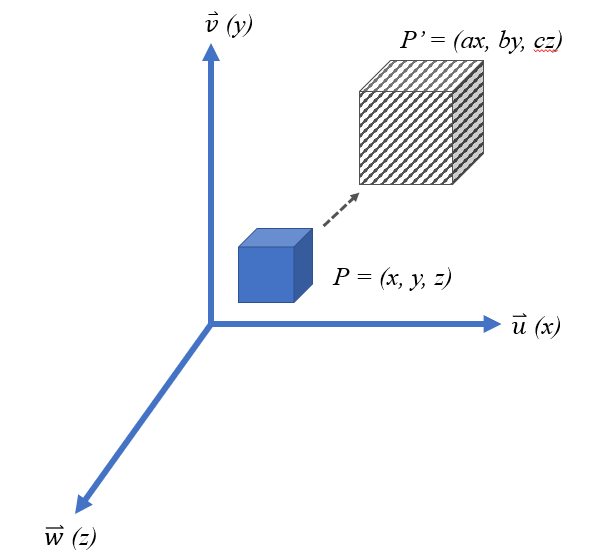
\includegraphics[scale=0.75]{scale}

We can similarly compose the scaling matrix creating a mapping from \\ $[x, y, c, 1] \rightarrow [ax, by, cz, 1]$:

\begin{equation}
    S_{a, b, c} = \begin{bmatrix}
        a & 0 & 0 & 0 \\
        0 & b & 0 & 0 \\
        0 & 0 & c & 0 \\
        0 & 0 & 0 & 1
    \end{bmatrix}
\end{equation}

\newpage

This matrix will perform a 3D scaling to any point $p = (x, y, z)$ by $(a, b, c)$

\begin{equation}
    p' = S_{a, b, c} = \begin{bmatrix}
        1 & 0 & 0 & a \\
        0 & 1 & 0 & b \\
        0 & 0 & 1 & c \\
        0 & 0 & 0 & 1
    \end{bmatrix}
    \begin{bmatrix}
        x \\
        y \\
        z \\
        1
    \end{bmatrix}
    = \begin{bmatrix}
        ax \\
        by \\
        cz \\
        1
    \end{bmatrix}
\end{equation}

\subsection{Rotation}
Note that both translation and scaling acts along an axis; however rotation in 3D is performed around a given axis, making it a bit more interesting than translation, scaling as well as its 2D counterpart. Given a 3D space, there exists an arbitrary number of possible axes.  We will begin by rotating about well defined axes and then around any arbitrary axes.

\subsection{Rotation (z-Axis)}
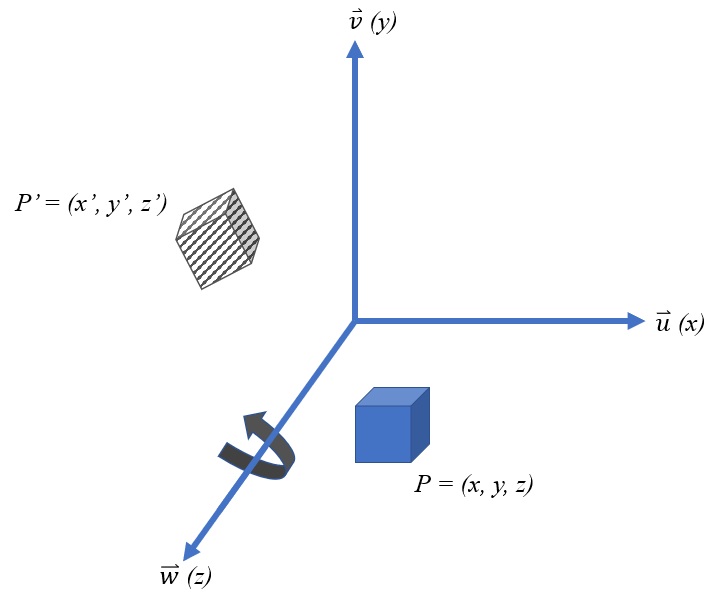
\includegraphics[scale=0.75]{zRotation}

We can image that the z-axis is the direction in which we view the 2D plane defined by $x$ and $y$ in the 2D scenario. To directly extend from the 2D rotational matrix, we first look at the rotation about the z-axis.

\begin{equation}
    R_{z, \theta} = \begin{bmatrix}
        \text{cos}(\theta) & -\text{sin}(\theta) & 0 & 0 \\
        \text{sin}(\theta) &  \text{cos}(\theta) & 0 & 0 \\
        0 & 0 & 1 & 0 \\
        0 & 0 & 0 & 1
    \end{bmatrix}
\end{equation}

If we examine the components in each axis, we see that the z-axis are all 0's which means that if we rotate about the z-axis, the z-coordinate does not change.

\newpage

Let's see how this would work in an example. Suppose we would like to rotate a point from $(1, 0, 0) \rightarrow (0, 1, 0)$. To accomplish this we need a $90^{\circ}$ rotation about the z-axis:

\begin{equation}
    \begin{aligned}
    p' = R_{z, 90^{\circ}}p
    &= \begin{bmatrix}
        \text{cos}(90^{\circ}) & -\text{sin}(90^{\circ}) & 0 & 0 \\
        \text{sin}(90^{\circ}) &  \text{cos}(90^{\circ}) & 0 & 0 \\
        0 & 0 & 1 & 0 \\
        0 & 0 & 0 & 1
    \end{bmatrix}
     \begin{bmatrix}
        1 \\
        0 \\
        0 \\
        1
    \end{bmatrix} \\
    &= \begin{bmatrix}
        0 & -1 & 0 & 0 \\
        1 & 0  & 0 & 0 \\
        0 & 0  & 1 & 0 \\
        0 & 0  & 0 & 1
    \end{bmatrix}
     \begin{bmatrix}
        1 \\
        0 \\
        0 \\
        1
    \end{bmatrix} \\
    &= \begin{bmatrix}
        0 \\
        1 \\
        0 \\
        1
    \end{bmatrix}
    \end{aligned}
\end{equation}

\subsection{Rotation (x-Axis)}
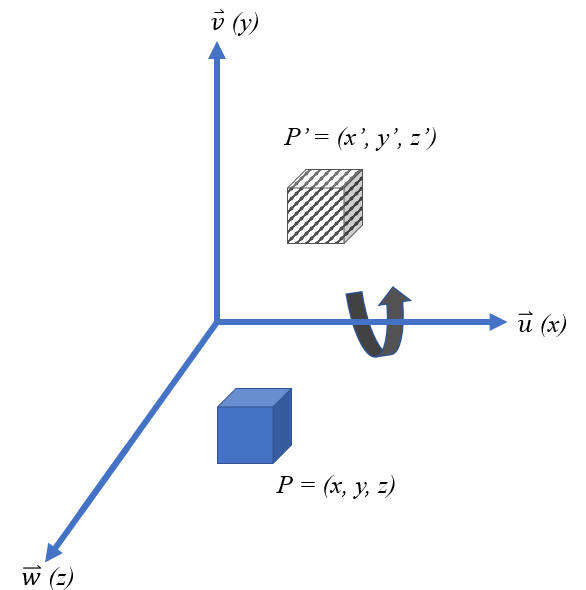
\includegraphics[scale=0.75]{xRotation}

To begin, rotating about the x-axis is similar that rotating about the z-axis in that the rotation still follows the right-hand-rule. Note that the right hand rule in this case curls towards the extension of the z-axis. To construct the rotational matrix for x-axis, we must observe that the x-component (by definition of rotation about the x-axis) cannot change. Hence, we have the constraint the components affected by the x-component must not change:

\begin{equation}
    R_{x, \phi} = \begin{bmatrix}
        1 & 0 & 0 & 0 \\
        0 & \text{cos}(\phi) & -\text{sin}(\phi) & 0 \\
        0 & \text{sin}(\phi) &  \text{cos}(\phi) & 0 \\
        0 & 0 & 0 & 1
    \end{bmatrix}
\end{equation}

\newpage

Now, suppose we would like to rotate a point from $(0, 1, 0) \rightarrow (0, 0, 1)$. To accomplish this we need a $90^{\circ}$ rotation about the x-axis:

\begin{equation}
    \begin{aligned}
    p' = R_{z, 90^{\circ}}p
    &= \begin{bmatrix}
        1 & 0 & 0 & 0 \\
        0 & \text{cos}(90^{\circ}) & -\text{sin}90^{\circ}) & 0 \\
        0 & \text{sin}(90^{\circ}) &  \text{cos}(90^{\circ}) & 0 \\
        0 & 0 & 0 & 1
    \end{bmatrix}
     \begin{bmatrix}
        0 \\
        1 \\
        0 \\
        1
    \end{bmatrix} \\
    &= \begin{bmatrix}
        1 & 0 &  0 & 0 \\
        0 & 0 & -1 & 0 \\
        0 & 1 &  0 & 0 \\
        0 & 0 &  0 & 1
    \end{bmatrix}
     \begin{bmatrix}
        0 \\
        1 \\
        0 \\
        1
    \end{bmatrix} \\
    &= \begin{bmatrix}
        0 \\
        0 \\
        1 \\
        1
    \end{bmatrix}
    \end{aligned}
\end{equation}


\subsection{Rotation (y-Axis)}
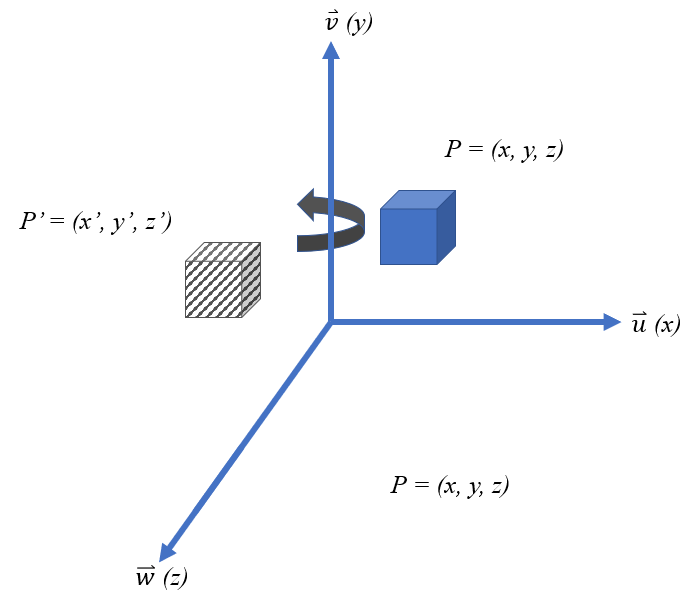
\includegraphics[scale=0.75]{yRotation}

Now we would imagine that the extension to the y-axis would be similar to that of the x-axis and z-axis. We know that to construct the rotational matrix for y-axis, we must observe that the y-component (again by definition of rotation about the y-axis) cannot change:

\begin{equation}
    R_{y, \psi} = \begin{bmatrix}
        \text{cos}(\psi)    & 0     & -\text{sin}(\psi) & 0 \\
        0                   & 1     &  0                & 0 \\
       \text{sin}(\psi)     & 0     &  \text{cos}(\psi) & 0 \\
        0                   & 0     &  0                & 1
    \end{bmatrix}
\end{equation}

\newpage

Now, suppose we would like to rotate a point from $(0, 0, 1) \rightarrow (1, 0, 0)$. To accomplish this we need a $90^{\circ}$ rotation about the y-axis:

\begin{equation}
    \begin{aligned}
    p' = R_{y, 90^{\circ}}p
    &= \begin{bmatrix}
        \text{cos}(90^{\circ})    & 0     & -\text{sin}(90^{\circ}) & 0 \\
        0                         & 1     &  0                      & 0 \\
       \text{sin}(90^{\circ})     & 0     &  \text{cos}(90^{\circ}) & 0 \\
        0                         & 0     &  0                      & 1
    \end{bmatrix}
     \begin{bmatrix}
        0 \\
        0 \\
        1 \\
        1
    \end{bmatrix} \\
    &= \begin{bmatrix}
        0 & 0 & -1 & 0 \\
        0 & 0 &  0 & 0 \\
        1 & 0 &  0 & 0 \\
        0 & 0 &  0 & 1
    \end{bmatrix}
     \begin{bmatrix}
        0 \\
        0 \\
        1 \\
        1
    \end{bmatrix} \\
    &= \begin{bmatrix}
        -1 \\
        0 \\
        0 \\
        1
    \end{bmatrix}
    \end{aligned}
\end{equation}

Notice that the result is actually incorrect; we have turned the wrong direction! Hence technically, we needed to turn $-90^{\circ}$. However, this is inconvenient, so instead, we set the z-component of the first row to be $\text{sin}(\psi)$ and the z-component of the first column to be $-\text{sin}(\psi)$ to produce a rotation matrix that adheres to the right-hand-rule.

\begin{equation}
    R_{y, \psi} = \begin{bmatrix}
        \text{cos}(\psi)    & 0     & \text{sin}(\psi) & 0 \\
        0                   & 1     &  0                & 0 \\
       -\text{sin}(\psi)     & 0     &  \text{cos}(\psi) & 0 \\
        0                   & 0     &  0                & 1
    \end{bmatrix}
\end{equation}

\newpage

Now if we were to reapply the rotation about the y-axis, we expect to get the correct results of $(0, 0, 1) \rightarrow (1, 0, 0)$:

\begin{equation}
    \begin{aligned}
    p' = R_{y, 90^{\circ}}p
    &= \begin{bmatrix}
        \text{cos}(90^{\circ})    & 0     & \text{sin}(90^{\circ}) & 0 \\
        0                         & 1     &  0                      & 0 \\
       -\text{sin}(90^{\circ})    & 0     &  \text{cos}(90^{\circ}) & 0 \\
        0                         & 0     &  0                      & 1
    \end{bmatrix}
     \begin{bmatrix}
        0 \\
        0 \\
        1 \\
        1
    \end{bmatrix} \\
    &= \begin{bmatrix}
        0 & 0 &  1 & 0 \\
        0 & 0 &  0 & 0 \\
       -1 & 0 &  0 & 0 \\
        0 & 0 &  0 & 1
    \end{bmatrix}
     \begin{bmatrix}
        0 \\
        0 \\
        1 \\
        1
    \end{bmatrix} \\
    &= \begin{bmatrix}
        1 \\
        0 \\
        0 \\
        1
    \end{bmatrix}
    \end{aligned}
\end{equation}

\subsection{Rotation About An Arbituary Axis}

Suppose we would like to rotate an arbitrary axis by an angle $\alpha$ where the axis is defined by a point $q = (q_x, q_y, q_z)$ and a vector $\overrightarrow{v} = <v_x, v_y, v_z>$. To rotate by $\alpha$ along this axis, we need to massage the axis to a known axis (namely the z-axis as it is the most standard one). Once it is co-linear with the known axis, we can rotate by $\alpha$ and massage the to the original position.

(1) As rotations operate with respect to the origin, we begin by translation the axis and the points by the offset of $\overrightarrow{T} = O-q = <0-q_x, 0-q_y, 0-q_z>$, we will generically refers to this as $\overrightarrow{T} = <t_x, t_y, t_z>$:

\begin{equation}
    T_{t_x, t_y, t_z} =
     \begin{bmatrix}
        1 & 0 & 0 & t_x \\
        0 & 1 & 0 & t_y \\
        0 & 0 & 1 & t_z \\
        0 & 0 & 0 & 1
    \end{bmatrix}
\end{equation}

\newpage

(2) Next we need to transform the points and the axis such that it is co-planar with a known plane (namely, y-z plane). We then rotate about the y-axis by some angle $\psi$ such that it is co-planar to the y-z plane:

\begin{equation}
    R_{y, \psi} =
     \begin{bmatrix}
        \text{cos}(\psi)  & 0 & \text{sin}(\psi) & 0 \\
        0 & 1 & 0 & 0 \\
        -\text{sin}(\psi) & 0 & \text{cos}(\psi) & 0 \\
        0 & 0 & 0 & 1
    \end{bmatrix}
\end{equation}

However, what is $\psi$ exactly? Is there a way to know know what $\psi$ is? If we look at it geometrically, we can decompose the vector $\overrightarrow{v}$ into it's components $<v_x, v_y, v_z>$. We can see that to rotate $\overrightarrow{v}$ to the y-z plane, the angle must be $\theta=\text{tan}^{-1}(\frac{v_x}{v_z})$ (which also aligns with our conclusion that the y-component should not be affected.

Notice that we have rotated in the opposite direction. In this case, we will need to rewrite $\psi$ as the following:

\begin{equation}
    \psi = 360^{\circ}-\text{tan}^{-1}(\frac{v_x}{v_z}) = -\theta
\end{equation}

(3) Now that we are co-planar with the y-z plane, we will need to rotate about the x-axis by an angle $\phi$ to become co-linear with the z-axis:

\begin{equation}
    R_{x, \phi} = \begin{bmatrix}
        1 & 0 & 0 & 0 \\
        0 & \text{cos}(\phi) & -\text{sin}(\phi) & 0 \\
        0 & \text{sin}(\phi) &  \text{cos}(\phi) & 0 \\
        0 & 0 & 0 & 1
    \end{bmatrix}
\end{equation}

Again, we will need to figure out what $\phi$ is. Since we are co-planar with y-z, there is no x-component (which is good since we will be rotating about the x-axis). Note that we have rotated the vector about the y-axis, this is a transformation of $\overrightarrow{v}$'s z-component using $v_x$ and $v_z$. The new $v_z' = \sqrt{v_x^2+v_z^2}$. Since the y-component remains unchanged, we can again apply the same geometric relation to obtain:

\begin{equation}
    \phi = \text{tan}^{-1}(\frac{v_y}{v_z'}) = \text{tan}^{-1}(\frac{v_y}{\sqrt{v_x^2+v_z^2}})
\end{equation}

(4) At this point, we are now co-linear with the z-axis. Hence, we can rotate by $\alpha$ using the z-axis rotation matrix:

\begin{equation}
    R_{z, \alpha} = \begin{bmatrix}
        \text{cos}(\alpha) & -\text{sin}(\alpha) & 0 & 0 \\
        \text{sin}(\alpha) &  \text{cos}(\alpha) & 0 & 0 \\
        0 & 0 & 1 & 0 \\
        0 & 0 & 0 & 1
    \end{bmatrix}
\end{equation}

(5) Since we have centered ourselves at the origin, we must rotate and translate back to the original frame of reference. We can simply use the inverse of our translation $T^{-1}_{t_x, t_y, t_z}$, $R^{-1}_{y, \psi}$, $R^{-1}_{x, \phi}$.

We arrive at our final set of transformation $g$ where $g$ is some global transformation matrix we may apply generically to any set of points:

\begin{equation}
    g = T^{-1}_{t_x, t_y, t_z}
        R^{-1}_{y, \psi}
        R^{-1}_{x, \phi}
        R_{z, \alpha}
        R_{x, \phi}
        R_{y, \psi}
        T_{t_x, t_y, t_z}
\end{equation}

Note that the order in which we apply the matrices matter! The new set of points $p'$ will simply be $p' = gp$.

\section{Degrees of Freedom}
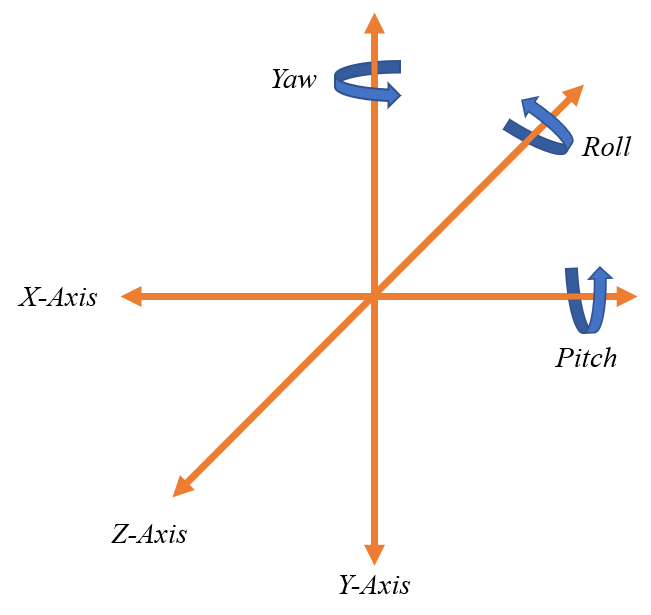
\includegraphics[scale=0.75]{DOF}

Now that we are able to translate, scale, and rotate in 3 dimensional space, we notice that there exists six degrees of freedom (DoF). The degrees of freedom of an object refers to the number of ways by which it can move. For 3 dimensions, the six degrees of freedom include:

\begin{enumerate}
    \item Translating along x-axis
    \item Translating along y-axis
    \item Translating along z-axis
    \item Rotating about x-axis (pitch)
    \item Rotating about y-axis (yaw)
    \item Rotating about z-axis (roll)
\end{enumerate}

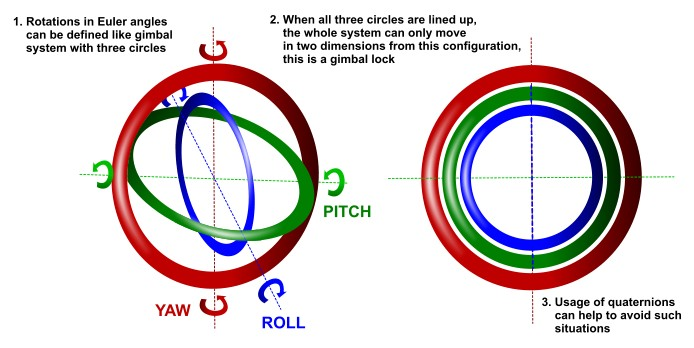
\includegraphics[scale=0.5]{gimballock}

However, the degrees of freedom are not as free as one would think. Suppose we represent the orientation (or pose) of an object (e.g. an airplane) by its position (x, y, z) and three gimbals (rings representing the rotation about x, y, and z-axis) in 3D space.

If one were to pitch the object $90^\circ$ or $-90^\circ$ (rotation about the x-axis), the z-axis of the object would align with its y-axis. If we now roll the object (rotation about the z-axis, now aligned with y-axis), we in fact induce yaw! This phenomenon is known as Gimbal Lock, where two gimbals are aligned parallel with each other causing a loss of a degree of freedom.

This phenomenon is possible for any three parameter representation of rotation (e.g. x, y, z rotation matrices, also known as Euler angles). To avoid this phenomenon, one would need a 4 parameter representation (e.g. quaternions).

\end{document}